% Three places for a model in an analysis: it writes code (keep), it is an
% instrument whose output enters only through a validation step (measure),
% or it produces the answer (avoid).
% ---------------------------------------------------------------------------
% style.tex --- shared preamble for every figure in book/figures/tikz/
%
% One style for all figures: Latin Modern, thin black lines, a light grey
% fill, and one accent colour used only to mark what is untrusted or wrong.
% Build with scripts/build_figures.sh; see book/figures/README.md.
% ---------------------------------------------------------------------------
\documentclass[tikz,border=6pt]{standalone}
\usepackage[T1]{fontenc}
\usepackage{lmodern}
\usetikzlibrary{arrows.meta,positioning,shapes.geometric,calc,fit,backgrounds}

\hyphenpenalty=10000   % short lines in boxes: ragged, never hyphenated

\definecolor{lightgrey}{gray}{0.92}
\definecolor{accent}{HTML}{9B2D20}

\tikzset{
  every picture/.style={
    line width=0.6pt,
    font=\small,
    >={Stealth[length=5pt,width=4pt]},
    node distance=14pt and 24pt,
  },
  % shapes
  box/.style={draw, rectangle, inner xsep=8pt, inner ysep=5pt,
              minimum height=22pt, align=center},
  grey/.style={box, fill=lightgrey},
  rounded/.style={box, rounded corners=9pt},
  decision/.style={draw, diamond, aspect=2.4, inner sep=1.5pt, align=center},
  group/.style={draw, dashed, rounded corners=5pt, inner sep=7pt},
  % text
  tag/.style={font=\footnotesize, align=center, inner sep=2pt},
  note/.style={font=\footnotesize\itshape, align=center, inner sep=2pt},
  code/.style={font=\small\ttfamily},
  codetag/.style={font=\footnotesize\ttfamily, align=center, inner sep=2pt},
  title/.style={font=\small\scshape, align=center, inner sep=2pt},
  % lines
  arrow/.style={->},
  back/.style={->, dashed},
  thin/.style={line width=0.4pt, gray},
  % the one accent, for what is untrusted, wrong or missing
  bad/.style={accent},
  badbox/.style={box, draw=accent, text=accent},
}

\begin{document}
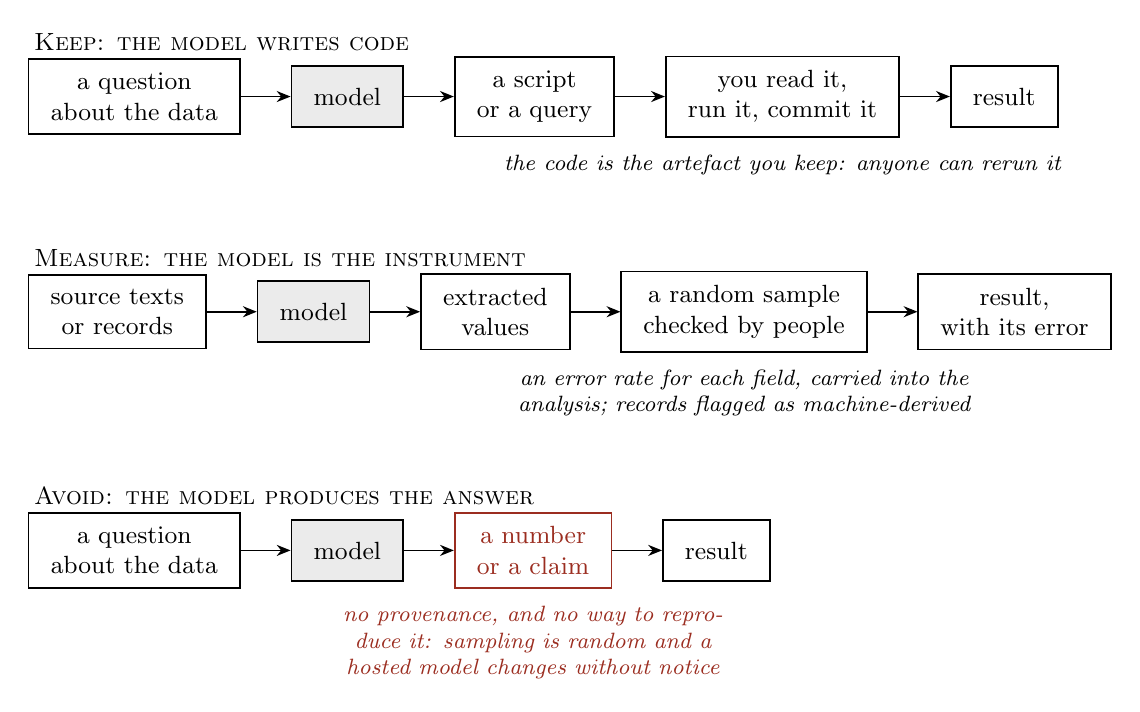
\begin{tikzpicture}[node distance=10pt and 18pt]
  \node[title, anchor=west] (t1) at (0,0) {Keep: the model writes code};
  \node[box, below=6pt of t1.west, anchor=north west] (q1) {a question\\about the data};
  \node[grey, right=of q1] (m1) {model};
  \node[box, right=of m1] (code) {a script\\or a query};
  \node[box, right=of code] (run) {you read it,\\run it, commit it};
  \node[box, right=of run] (r1) {result};
  \draw[->] (q1) -- (m1); \draw[->] (m1) -- (code); \draw[->] (code) -- (run); \draw[->] (run) -- (r1);
  \node[note, below=4pt of run] {the code is the artefact you keep: anyone can rerun it};

  \node[title, anchor=west] (t3) at (0,-78pt) {Measure: the model is the instrument};
  \node[box, below=6pt of t3.west, anchor=north west] (q3) {source texts\\or records};
  \node[grey, right=of q3] (m3) {model};
  \node[box, right=of m3] (ext) {extracted\\values};
  \node[box, right=of ext] (val) {a random sample\\checked by people};
  \node[box, right=of val] (r3) {result,\\with its error};
  \draw[->] (q3) -- (m3); \draw[->] (m3) -- (ext); \draw[->] (ext) -- (val); \draw[->] (val) -- (r3);
  \node[note, below=4pt of val, text width=200pt] {an error rate for each field, carried into the analysis; records flagged as machine-derived};

  \node[title, anchor=west] (t2) at (0,-164pt) {Avoid: the model produces the answer};
  \node[box, below=6pt of t2.west, anchor=north west] (q2) {a question\\about the data};
  \node[grey, right=of q2] (m2) {model};
  \node[badbox, right=of m2] (num) {a number\\or a claim};
  \node[box, right=of num] (r2) {result};
  \draw[->] (q2) -- (m2); \draw[->] (m2) -- (num); \draw[->] (num) -- (r2);
  \node[note, below=4pt of num, text width=180pt, text=accent] {no provenance, and no way to reproduce it: sampling is random and a hosted model changes without notice};
\end{tikzpicture}
\end{document}
